\documentclass{article}

\usepackage[french]{babel}
\usepackage[utf8]{inputenc}
\usepackage{lipsum}
\usepackage{amsmath, amssymb, amsthm, graphicx}
\usepackage{tikz}
\usepackage{multicol}
\usepackage[hidelinks]{hyperref}
\usepackage[backend=biber,style=numeric,sorting=none]{biblatex} % Use biblatex for numerical citations
\addbibresource{refs.bib} % Ensure refs.bib is your bibliography file
\usepackage{caption}
\captionsetup{font=footnotesize}
\usepackage{multirow}
\usepackage{adjustbox}
\usepackage{listings}
\usepackage{float} % Removed as it may conflict with other packages

% Define the \field command to avoid errors
\newcommand{\field}[2][]{\textbf{#1#2}}

\graphicspath{{img/}}
\setlength{\parindent}{0pt}

\newtheorem{theorem}{Théorème}

%%%%%%%%%%%%%%%% Lengths %%%%%%%%%%%%%%%%
\setlength{\textwidth}{17.5cm}
\setlength{\evensidemargin}{-1cm}
\setlength{\oddsidemargin}{-1cm}
\setlength{\topmargin}{-2cm}
\setlength{\textheight}{24cm}


%%%%%%%%%%%%%%%% Variables %%%%%%%%%%%%%%%%
\def\projet{6}
\def\titre{Résolution d'équations différentielles ordinaires et ses applications}
\def\groupe{4}
\def\equipe{4}
\def\responsible{Melissa Colin}
\def\secretary{Alexandre De Gendre}
\def\others{Cécile Barrat, Yahya Bel Ajjam}

\begin{document}

%%%%%%%%%%%%%%%% Header %%%%%%%%%%%%%%%%
\begin{minipage}{0.98\textwidth}
  \vskip 0mm
    { \begin{tabular}{p{7.5cm}}
      {\bfseries \sffamily
        Projet \projet} \\ 
      {\itshape \titre}
    \end{tabular}}
  \hfill 
  \fbox{\begin{tabular}{l}
      {~\hfill \bfseries \sffamily Groupe \groupe\ - Équipe \equipe
        \hfill~} \\[2mm] 
      Responsable : \responsible \\
      Secrétaire : \secretary \\
      Codeurs : \others
    \end{tabular}}
  \vskip 4mm ~

  ~~~\parbox{0.95\textwidth}{\small \textit{Résumé~:} \sffamily 

  Ce projet a permis de développer un solveur d'équations différentielles ordinaires (EDO) basé sur la méthode de Cauchy. L'algorithme a été testé sur diverses modélisations, notamment l'évolution de la population d'un ensemble d'individus et le filtrage d'images via l'équation de la chaleur et le filtre de Perona et Malik. Les résultats montrent que les méthodes d'intégration numérique sont efficaces pour résoudre des EDO, bien que certaines soient mieux adaptées à des équations spécifiques.
  }
  \vskip 1mm ~
\end{minipage}


%%%%%%%%%%%%%%%%% TEMPLATE %%%%%%%%%%%%%%%%
\section{Introduction}
Ce travail s'intéresse aux méthodes de résolution d'équations différentielles ordinaires (EDO). 
Ces équations sont très présentes dans de nombreux domaines et permettent de modéliser des systèmes complexes relativement simplement.\\
Ainsi, la résolution d'un problème de Cauchy a été implémentée en utilisant différentes méthodes d'intégration numérique. L'algorithme a ensuite été éprouvé sur différentes modélisations de l'évolution de la population d'un ensemble d'individus ainsi que le filtrage d'images en utilisant l'équation de la chaleur et le filtre de Perona et Malik.\\
La méthodologie mise en place pour résoudre les équations différentielles sera présentée, suivie des résultats obtenus et de leur discussion. Enfin, une conclusion sur les résultats obtenus et les perspectives d'amélioration de ce travail sera proposée.

\section{Méthodologie}
Dans cette partie, les algorithmes développés pour résoudre les équations différentielles seront détaillés. 
Le fonctionnement du problème de Cauchy ainsi que les différentes méthodes d'intégration numérique implémentées pour le résoudre seront expliqués. 
Ensuite, la modélisation de l'évolution de la population d'un ensemble d'individus au cours du temps sera présentée, en utilisant les modèles de Malthus et de Verhulst ainsi que le système proie-prédateur de Lotka-Volterra.
Enfin, le filtrage d'images en utilisant l'équation de la chaleur et le filtre de Perona et Malik sera abordé.

\subsection{Résolution d'équations différentielles}
Quatre méthodes de résolution d'équations différentielles ont été implémentées pour résoudre un problème de Cauchy.\\
Un problème de Cauchy est un système d'équations différentielles avec conditions initiales où la dérivée \(y'\) est fonction \(f\) de \(y\) avec \(f\) de la forme : \( y'(t) = f\bigl(y(t),\,t\bigr) \)\\
Les différentes méthodes implémentées sont toutes des méthodes à un pas de la forme suivante : \( y_{n+1} = y_n + h_n \,\Phi\bigl(y_n, t_n, h_n\bigr) \)\\ 
Pour résoudre ce problème de Cauchy, un solveur Cauchy a été créé, réunissant quatre méthodes explicites : Euler, point-milieu, Heun et Runge–Kutta 4. Chacune est représentée par une fonction \texttt{step} indépendante, appelée par \textit{meth\_n\_step} qui exécute \(N\) pas de taille \(h\). Une boucle adaptative \textit{meth\_epsilon} double \(N\) et divise \(h\) jusqu’à ce que la norme de la différence entre deux raffinements successifs atteigne la tolérance \(\varepsilon\).  
Les états sont mémorisés sous la forme d’un couple de tableaux \((\mathbf t,\mathbf y)\) : \((t_n)_n\) regroupe les abscisses où la solution est évaluée, et \((y_n)_n\) contient les valeurs approchées retournées par le solveur.\\ \\

Les résultats obtenus ont été testés et visualisés avec deux équations différentielles différentes dont la solution pouvait être calculée manuellement :
\begin{itemize}
  \item En dimension 1 : \( \begin{cases} y(0) = 1 \\ y'(t) = \dfrac{y(t)}{1 + t^2} \end{cases} \)
  \item En dimension 2 : \( y(t) = \begin{bmatrix} y_1(t) \\ y_2(t) \end{bmatrix} \quad \text{avec} \quad \begin{cases} y(0) = \begin{bmatrix} 1 \\ 0 \end{bmatrix} \\ y'(t) = \begin{bmatrix} -y_2(t) \\ y_1(t) \end{bmatrix} \end{cases} \)
\end{itemize}
Pour visualiser les résultats, le champ des tangentes de l'équation différentielle et ses solutions pour différentes conditions initiales ont été tracés en figures~\ref{fig:cauchy_on_tan_field_f_1_runge_kutta_4} et~\ref{fig:cauchy_on_tan_field_f_2_runge_kutta_4}. De plus, ceci permet d'estimer l'impact de petites variations sur les conditions initiales.\\
La précision (norme de la différence entre deux raffinements successifs) des méthodes d'intégration numérique a également été étudiée en fonction du nombre d'itérations \(N\) sur les deux équations différentielles. Ceci afin de comparer les méthodes entre elles et de déterminer la méthode la plus efficace pour chaque équation. Ces résultats sont présentés dans la figure~\ref{fig:precision}.
\subsection{Modélisation de l'évolution de la population}
Pour éprouver l'algorithme de résolution d'équations différentielles, la modélisation de l'évolution de la population d'un ensemble d'individus au cours du temps a été étudiée.\\ \\
Si la fonction $N(t)$ représente la variation de la population d’un ensemble d’individus au cours du temps, l’évolution de cette population peut être modélisée par deux modèles différents~: le \textbf{modèle de Malthus} (équation~\ref{eq:malthus}) et le \textbf{modèle de Verhulst} (équation~\ref{eq:verhulst}).\\
\begin{minipage}{0.48\textwidth}
  \begin{equation}
    \label{eq:malthus}
    \frac{dN(t)}{dt} = \gamma N(t)
  \end{equation}
\end{minipage}
\hfill
\begin{minipage}{0.48\textwidth}
  \begin{equation}
    \label{eq:verhulst}
    \frac{dN(t)}{dt} = \gamma N(t) \left(1 - \frac{N(t)}{\kappa}\right)
  \end{equation}
  \\
\end{minipage}

Dans l'équation du modèle de Malthus, la constante $\gamma$ correspond au taux de croissance net (naissance - mort). Ce modèle suppose que la croissance de la population est proportionnelle à la taille de la population actuelle. La population croît de manière exponentielle si $\gamma$ est positif, et décroît de la même façon si $\gamma$ est négatif.\\
Le modèle de Verhulst, quant à lui, introduit la constante $\kappa$, représentant la capacité de charge de l'environnement. Pour de petites populations, ce modèle se rapproche de celui de Malthus. Cependant, lorsque $N$ $\approx$ $\kappa$, la croissance de la population ralentit et converge vers la valeur maximale $\kappa$.
\\ \\
La méthode de Runge-Kutta a été utilisée pour simuler la croissance de la population de bactéries en appliquant les modèles de Malthus et de Verhulst, permettant ainsi une comparaison des résultats. Une population initiale de 100 Unités Formant Colonie (UFC), un taux de croissance de 0,85 par heure et une capacité limite fixée à 9000 UFC, d'après les données fournies par le laboratoire de microbiologie de l'INSA Lyon~\cite{insa2024microorganismes}, ont servi de base à cette simulation. Les résultats obtenus sont présentés dans la figure~\ref{fig:population_models}.\\ \\
Pour approfondir l'étude, un écosystème avec deux espèces interagissant entre elles, modélisé par le système proie-prédateur, peut être envisagé. Le modèle de Lotka-Volterra, défini par les équations~\ref{eq:lotka-volterra}, constitue une approche classique pour représenter ce type de dynamique.
\begin{equation}
  \label{eq:lotka-volterra}
  \begin{cases}
    \frac{dN(t)}{dt} = N(t) (a-bP(t)) \\\
    \frac{dP(t)}{dt} = P(t) (cN(t)-d)
  \end{cases}, \quad a;b;c;d > 0
\end{equation}
Ce système utilise les constantes $a$, $b$, $c$ et $d$ qui représentent respectivement le taux de croissance des proies, le taux de prédation, le taux de croissance et de mortalité des prédateurs\\
Il modélise une croissance des proies $N(t)$ proportionnelle à leur taux de croissance $a$ et inversement proportionnelle à la population de prédateurs $P(t)$. La croissance des prédateurs $P(t)$ est proportionnelle à la population de proies $N(t)$ et inversement proportionnelle à leur taux de mortalité $d$.\\ \\
L'évolution de la population de proies et de prédateurs a été simulée en utilisant le modèle de Lotka-Volterra avec la méthode de Runge-Kutta. L'interaction entre une population de protozoaires : \textit{Paramecium caudatum} (proies) et \textit{Didinium nasutum} (prédateurs), comme décrite dans les expériences pionnières de Georgy Gause~\cite{strauss2021gauser}, a été étudiée. Les paramètres du modèle de Lotka-Volterra ont été estimés à partir des données expérimentales : $a$, le taux de croissance des proies est de $1.10$, $b$, le taux de prédation est de $0.08$, $c$, le taux de reproduction des prédateurs par proie consommée est de $0.08$ et $d$, le taux de mortalité naturel des prédateurs est de $0.89$. Une population initiale de $1.66$ pour les proies et $0.12$ pour les prédateurs a été utilisée. \\ \\
Les variations des deux populations au cours du temps ont été tracées. Les solutions du système de Lotka-Volterra étant généralement périodiques, des cycles ont été observés. Les variations \((N(t), P(t))\) (\textit{portrait de phase}) au cours du temps ont été représentées, mettant en évidence les solutions périodiques du système. Les solutions constantes correspondent aux points d'équilibre où les populations de proies et de prédateurs ne changent pas. Ces points d'équilibre sont donnés par \((N, P) = (0, 0)\) et \((N, P) = \left(\frac{d}{c}, \frac{a}{b}\right)\), comme présenté dans la figure~\ref{fig:lotka_volterra}.\\ \\
Pour approfondir l'étude, l'impact de légères variations des paramètres du modèle de Lotka-Volterra sur les solutions du système a été analysé. Les solutions du système de Lotka-Volterra pour le cas précédent ont été tracées en ajoutant des variations sur les populations initiales de proies et de prédateurs de $\pm 0.01$. Ces variations sont présentées dans la figure~\ref{fig:lotka_volterra_variations}.\\ \\
Dans le contexte plus général des équations différentielles, les solutions peuvent adopter différents comportements en fonction des paramètres et des conditions initiales. Des \textbf{points fixes}, où les solutions convergent vers un état stable, des \textbf{cycles limites}, où les solutions deviennent périodiques, ou encore des phénomènes de \textbf{chaos}, où les solutions sont apériodiques et très sensibles aux conditions initiales, peuvent être observés. D'autres comportements incluent les \textbf{nœuds}, où les solutions convergent ou divergent linéairement, et les \textbf{foyers}, où les solutions convergent ou divergent de manière spirale~\cite{diener_sysdyn12}.
\subsection{Filtrage d'images}
Une image numérique (en échelle de gris) est un ensemble de pixels, chacun ayant une valeur d'intensité lumineuse. Celle-ci peut être modélisée par une fonction \( u(x,y) \) qui associe à chaque pixel \((x,y)\) une intensité réelle. Pour améliorer la qualité d'une image ou en extraire certaines caractéristiques, des opérations de filtrage, comme le filtrage par équation de la chaleur ou le filtrage de Perona et Malik, peuvent être appliquées.\\ \\

Le filtrage par équation de la chaleur consiste à faire évoluer l'image dans le temps selon l'équation de la chaleur~\ref{eq:heat_equation}~\cite{is104-perona}, qui modélise un lissage uniforme de l'image :
\begin{equation}
  \label{eq:heat_equation}
  \begin{cases}
  \dfrac{\partial u}{\partial t}(x,y,t) - \Delta u(x,y,t) = 0 \text{, pour } t>0 \\
  u(0,x,y) = u_0(x,y)
  \end{cases}
\end{equation}

où \( u_0(x,y) \) est l'image initiale, et \( \Delta u = \nabla \cdot \nabla u \) est le laplacien discrétisé à l'aide d'opérateurs de gradient et de divergence.\\
Pour implémenter cela, nous calculons le gradient ligne par ligne et colonne par colonne, ainsi que la divergence en utilisant la formule de la divergence discrète. Le laplacien est ainsi calculé en appliquant la divergence au gradient.\\
L’évolution temporelle de cette équation est intégrée numériquement via un schéma d’Euler explicite. Dans ce cadre, nous utilisons donc notre fonction \texttt{meth\_n\_step} avec la méthode d'Euler, la fonction d'entrée étant l'EDO par le calcul du laplacien de l’image.\\
L'équation de la chaleur est un bon point de départ pour le filtrage d'images, mais elle présente des inconvénients majeurs, notamment le flou des contours. En effet, l'équation de la chaleur lisse uniformément l'image, ce qui peut entraîner une perte d'informations importantes sur les bords et les détails. Pour remédier à cela, nous avons exploré le filtre de Perona-Malik, qui est une méthode de filtrage permettant de préserver les contours tout en lissant les zones homogènes de l'image. Cette méthode repose sur l'équation~\ref{eq:pm_equation}~\cite{is104-perona} :
\begin{equation}
  \label{eq:pm_equation}
  \begin{cases}
  \dfrac{\partial u}{\partial t}(x,y,t) = \nabla \cdot \left( f(x,y) \cdot \nabla u(x,y,t) \right), \text{ pour } t > 0 \\
  u(0,x,y) = u_0(x,y)
  \end{cases}
\end{equation}
où la fonction \( f(x,y) \in [0,1] \) module l’intensité du filtrage selon la norme du gradient de l’image initiale. Plus précisément, \( f \) est définie par \( f(x,y) = \exp\left( -\| \nabla F(x,y) \|^2 \right) \) avec \( F(x,y) \) représentant une convolution de l'image initiale \( u_0(x,y) \) avec une gaussienne de variance \( \sigma \), utilisée pour adoucir le calcul du gradient et élargir les zones de contours.

Pour intégrer cette équation sur 200 itérations avec un pas de temps \( \delta t = 0.2 \), la fonction \( f \) a été calculée par convolution gaussienne (\texttt{\\scipy.signal.convolve2d}, mode \texttt{symm} pour gérer les bords). Le calcul de la dérivée spatiale a été adapté pour inclure \( f \) dans le produit \( f \cdot \nabla u \), suivi de la divergence.

Ces deux méthodes de filtrage ainsi que la convolution gaussienne ont été appliquées à l'image \textit{camera} de \textit{skimage}~\cite{scikit-image-camera}, en utilisant la méthode d'Euler. Les résultats sont présentés dans la figure~\ref{fig:all_filters}.
Pour étudier l'impact de la fonction \( f \) sur le filtrage, la fonction de Perona-Malik a également été tracée en fonction de la norme du gradient de l'image initiale avec et sans gaussienne. Cette fonction est présentée dans la figure~\ref{fig:perona_malik_function}.

\section{Résultats et discussions}
Dans cette partie, nous allons présenter les résultats obtenus avec notre algorithme de résolution d'équations différentielles. Nous allons d'abord discuter des résultats obtenus avec le solveur Cauchy et les différentes méthodes d'intégration numérique. Ensuite, nous allons aborder les résultats obtenus avec la modélisation de l'évolution de la population d'un ensemble d'individus ainsi que le filtrage d'images.

\subsection{Résolution d'équations différentielles}
L'implémentation de Cauchy a apporté diverses contraintes nécessitant plusieurs ajustements au cours du projet. Un problème de convergence a été observé avec la méthode d'Euler, qui, en raison de sa lenteur, atteignait rapidement des valeurs de \(N\) très élevées. Cela entraînait des temps de calcul prolongés, des erreurs numériques, des valeurs de \(h\) extrêmement petites, voire des problèmes de mémoire. Pour résoudre ces difficultés, la valeur initiale de \(N\) a été adaptée en fonction de la méthode choisie, et celle de \(h\) ajustée en conséquence.
\begin{figure}[H]
  \begin{minipage}{0.65\textwidth}
    \centering
    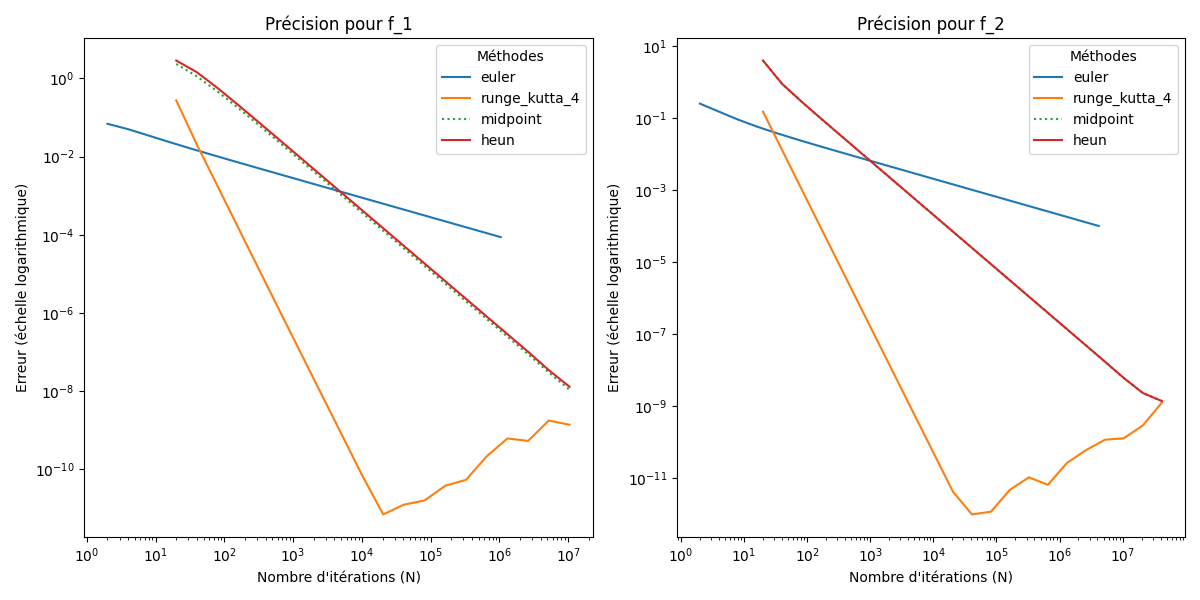
\includegraphics[width=\textwidth]{img/_bis.png}
    \captionof{figure}{Évolution de la précision en fonction du nombre d'itérations \(N\) pour chaque méthode d'intégration numérique (Euler, Runge-Kutta d'ordre 4, point milieu et Heun) pour \(f_1 = \frac{y}{1 + t^2}\) et \(f_2 = (y'_1, y'_2) = (-y_2, y_1)\). \\}
    \label{fig:precision}
  \end{minipage}
  \hfill
  \begin{minipage}{0.33\textwidth}
    La figure~\ref{fig:precision} illustre l'évolution de la précision des différentes méthodes d'intégration numérique en fonction du nombre d'itérations \(N\). \\
  On observe que la méthode d'Euler, d'ordre 1, est celle qui converge le plus lentement, avec une précision qui n'atteint pas la tolérance de \(10^{-4}\) même pour \(N = 10^7\) sur \(f_1\). En revanche, les méthodes de Heun et du point-milieu, toutes deux d'ordre 2, convergent plus rapidement, et à la même vitesse, atteignant la tolérance de \(10^{-8}\).
  \end{minipage}
\end{figure}
La méthode de Runge-Kutta d'ordre 4, quant à elle, converge rapidement, atteignant la tolérance de \(10^{-11}\) en dimension 1 et \(10^{-12}\) en dimension 2 pour \(N = 10^4\) sur \(f_1\) et \(N = 10^5\) sur \(f_2\). Cependant, elle diverge pour des valeurs de \(N\) plus élevées, ce qui est inattendu.\\ \\
Par ailleurs, des problèmes de stabilité et de mémoire liés à des fonctions complexes à résoudre ont été rencontrés. Des solutions égales à \textit{nan} ou \textit{inf} apparaissaient fréquemment, et les tableaux dépassaient la mémoire disponible. Pour y remédier, le stockage des données a été adapté en utilisant des \textit{numpy.array} au lieu de listes.
\begin{figure}[H]
  \centering
  \begin{minipage}{0.48\textwidth}
    \centering
    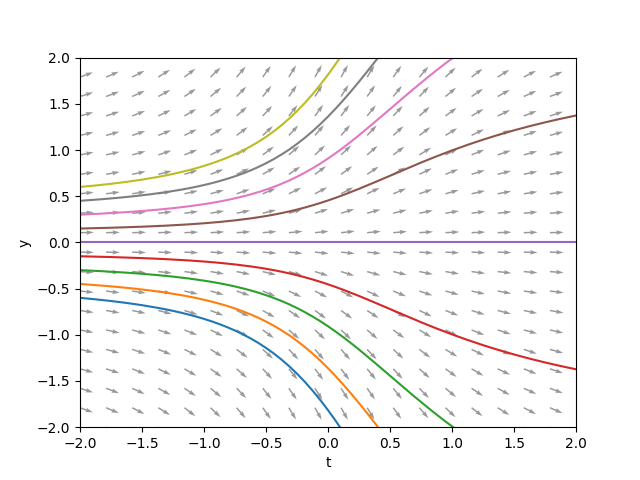
\includegraphics[width=0.7\textwidth]{img/cauchy_on_tan_field_f_1_runge_kutta_4.png}
    \caption{Champ des tangentes de $(E)$ $y' = \frac{y}{1 + t^2}$ (dimension 1) et solutions de $(E)$ pour différentes conditions initiales avec la méthode de Runge-Kutta d'ordre 4.}
    \label{fig:cauchy_on_tan_field_f_1_runge_kutta_4}
  \end{minipage}
  \hfill
  \begin{minipage}{0.48\textwidth}
    \centering
    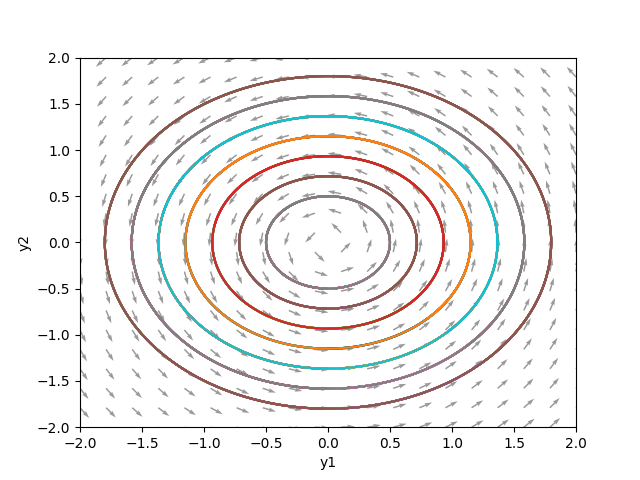
\includegraphics[width=0.7\textwidth]{img/cauchy_on_tan_field_f_2_runge_kutta_4.png}
    \caption{Champ des tangentes de $(E)$  $(y'_1, y'_2) = (-y_2, y_1)$ (dimension 2) et solutions de $(E)$ pour différentes conditions initiales avec la méthode de Runge-Kutta d'ordre 4.}
    \label{fig:cauchy_on_tan_field_f_2_runge_kutta_4}
  \end{minipage}
\end{figure}
Après ces multiples corrections, des résultats cohérents et intéressants ont été obtenus, bien que l'intervalle sur lequel la fonction est calculée fût trop faible. Pour résoudre ce problème et obtenir les résultats finaux, un paramètre d'entrée \texttt{t\_end} a été ajouté, permettant d'ajuster la valeur de \(h\). Les figures~\ref{fig:cauchy_on_tan_field_f_1_runge_kutta_4} et~\ref{fig:cauchy_on_tan_field_f_2_runge_kutta_4} illustrent le champ des tangentes des équations différentielles et les solutions des équations pour différentes conditions initiales en dimension 1 et 2.\\
Ces figures montrent que les solutions suivent de façon cohérente le champ des tangentes. Elles permettent également d'observer qu'une faible variation dans la position initiale peut avoir un fort impact sur le résultat final.

\subsection{Modélisation de l'évolution de la population}
L'algorithme de résolution d'équations différentielles a ensuite été appliqué pour modéliser l'évolution de la population d'un ensemble d'individus au cours du temps. Les modèles de Malthus et de Verhulst ont été étudiés en premier, suivis par le système proie-prédateur de Lotka-Volterra.
\begin{figure}[H]
  \begin{minipage}{0.48\textwidth}
    \centering
    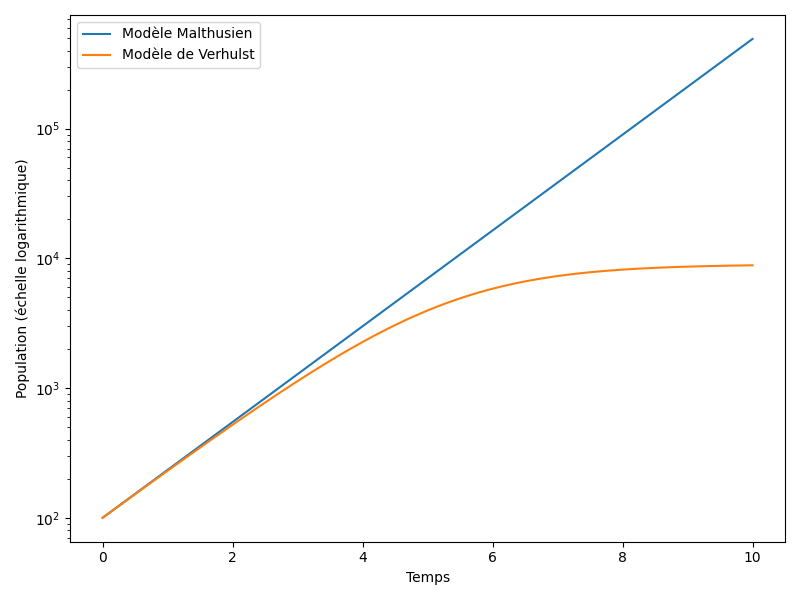
\includegraphics[width=\textwidth]{img/population_models.png}
    \captionof{figure}{Évolution de la population de bactéries en fonction du temps pour les modèles de Malthus et de Verhulst avec une population initiale de 100 UFC, un taux de croissance de 0,85 par heure et une capacité limite de 9000 UFC.}
    \label{fig:population_models}
    \end{minipage}
    \hfill
    \begin{minipage}{0.48\textwidth}
    Comme nous l'avions précédemment anticipé, nous pouvons observer figure~\ref{fig:population_models} que les deux modèles de Malthus et de Verhulst sont similaires pour de petites populations et croissent de manière exponentielle.
    Mais rapidement, on observe que lorsque la population augmente, là où le modèle de Malthus continue d'augmenter
    exponentiellement, le coefficient de régulation commence à avoir un impact sur la croissance dans le modèle de Verhulst, 
    où l'on voit la croissance de population ralentir jusqu'à converger vers la limite que l'on lui a imposée, à savoir 9000 UFC.
    Ces résultats sont cohérents avec les données fournies par le laboratoire de microbiologie de l'INSA Lyon~\cite{insa2024microorganismes} et montrent que le modèle de Verhulst est plus adapté pour modéliser la croissance de la population de bactéries dans un environnement limité.
    \end{minipage}
\end{figure}
Quant à nos résultats sur le système proie-prédateur de Lotka-Volterra présenté en figure~\ref{fig:lotka_volterra}, nous pouvons observer que l'évolution des populations est périodique avec une courbe d'évolution symétrique entre les proies et les prédateurs. Ce cycle est cohérent et suit les phases suivantes:\\
\begin{enumerate}
  \item La population de proies augmente en l'absence de prédateurs pour les chasser.
  \item Les prédateurs retrouvent des proies pour se nourrir, donc voient à leur tour leur population augmenter.
  \item Une fois que la proportion de prédateurs est devenue trop grande, la population de proies se met à baisser drastiquement jusqu'à atteindre 0.
  \item Les prédateurs trouvent alors de moins en moins de nourriture et commencent à périr jusqu'au dernier.
  \item Le cycle recommence.
\end{enumerate}
Cette notion de cycle est bien visible sur la figure~\ref{fig:lotka_volterra_variations} du diagramme de phase formant un cycle, et sur la représentation des courbes individuelles figure~\ref{fig:lotka_volterra}, où l'on voit les deux courbes évoluer périodiquement (période visible en pointillés sur l'axe des abscisses).
\begin{figure}[H]
  \centering
  \begin{minipage}{0.48\textwidth}
    \centering
    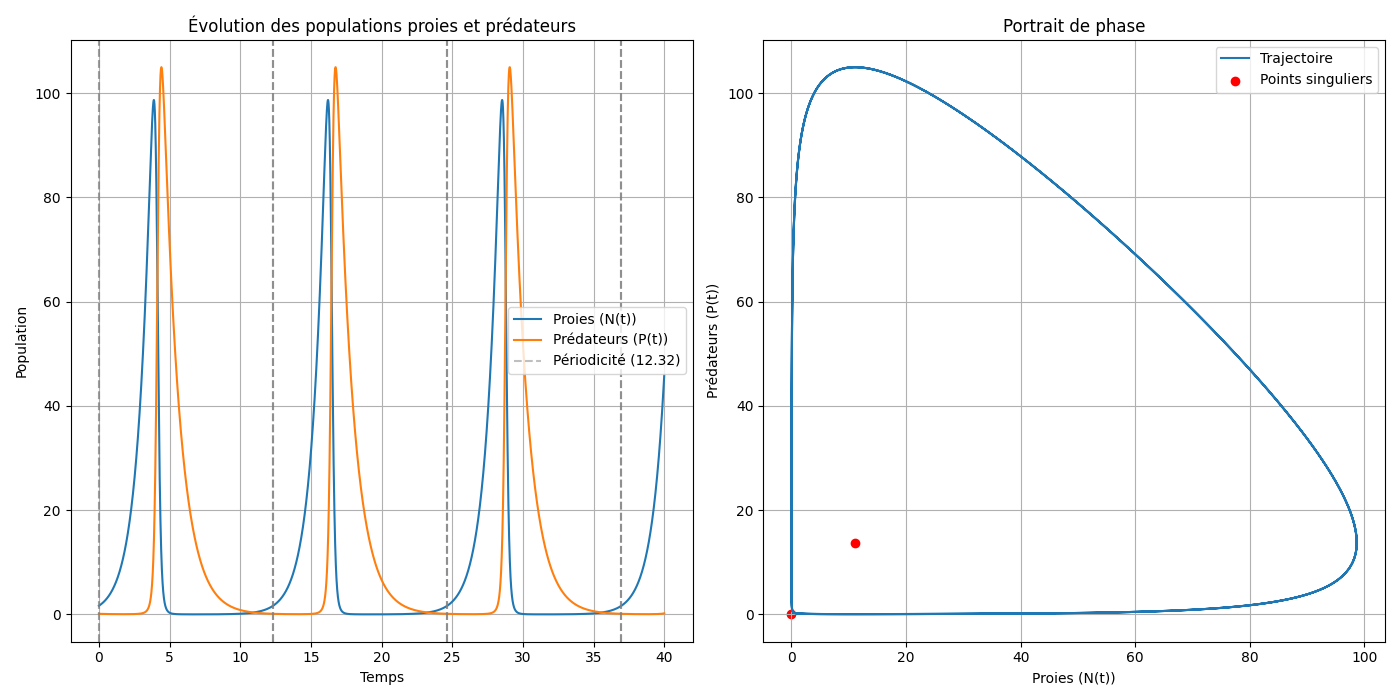
\includegraphics[width=\textwidth]{img/population_dynamics.png}
    \caption{Évolution de la population de proies et de prédateurs en fonction du temps pour le modèle de Lotka-Volterra avec la population \textit{Paramecium caudatum} (proies) et \textit{Didinium nasutum} (prédateurs) et portrait de phase.}
    \label{fig:lotka_volterra}
  \end{minipage}
  \hfill
  \begin{minipage}{0.48\textwidth}
    \centering
    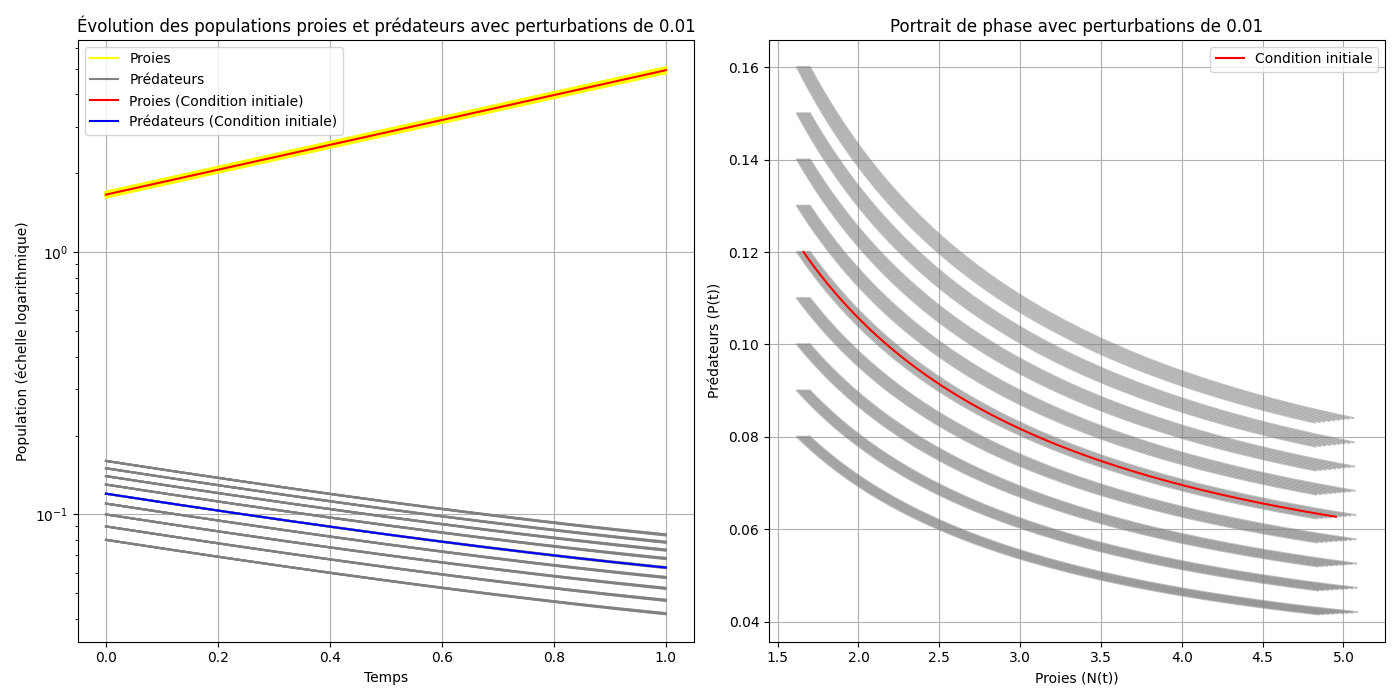
\includegraphics[width=\textwidth]{img/solutions_around_initial_zoom.png} % SI BESOIN : img/solutions_around_initial.png
    \caption{Évolution de la population de proies et de prédateurs en fonction du temps pour le modèle de Lotka-Volterra avec des variations sur les populations initiales de proies et de prédateurs de $\pm 0.01$.}
    \label{fig:lotka_volterra_variations}
  \end{minipage}
\end{figure}
La figure~\ref{fig:lotka_volterra_variations} montre que les variations des populations initiales de proies et de prédateurs ont un impact peu significatif sur l'évolution des populations au cours du temps dans notre contexte. En effet, même de petites variations dans les conditions initiales peuvent entraîner des différences de l'ordre de 10 dans le comportement du système mais n'impactent pas le cycle. Il pourrait être néanmoins pertinent de confirmer cette hypothèse sur d'autres populations avec des cycles différents. Cela pour souligner l'importance de la sensibilité aux conditions initiales dans les systèmes dynamiques, en particulier dans le contexte des modèles de Lotka-Volterra.\\ \\

Comme représenté sur la figure \ref{fig:lotka_volterra}, les points singuliers calculés pour notre système se situent à la fin du cycle lorsque les populations des prédateurs et des proies valent toutes deux 0. Ce qui est logique car c'est le moment où la population des proies peut commencer à ré-augmenter en l'absence de prédateurs après avoir chuté dû à un surplus de ces derniers, et simultanément le moment où la population des prédateurs ne peut plus descendre ayant atteint 0.\\
Les courbes ont la forme d'une exponentielle positive et négative dans les phases respectives d'augmentation et 
de diminution de population, ce qui est cohérent avec l'expression des dérivées dans le système. 

\subsection{Filtrage d'images}
\begin{figure}[H]
  \centering
  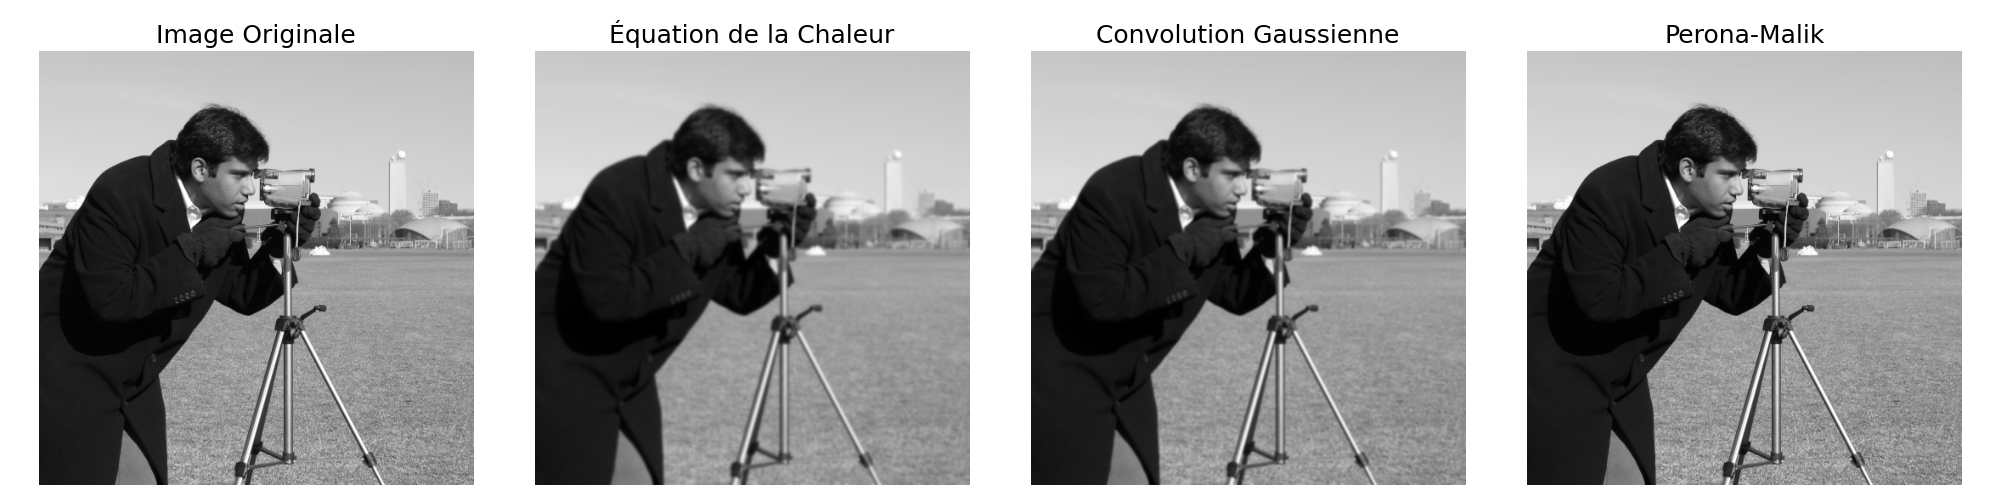
\includegraphics[width=\textwidth]{img/all_filters.png}
  \caption{Image \textit{camera} de \textit{skimage}~\cite{scikit-image-camera} origianle et avec l'équation de la chaleur, convolution gaussienne et le filtrage de Perona-Malik pour 200 itérations avec un pas de 0.2 et $\sigma = 1$.}
  \label{fig:all_filters}
\end{figure}
Nous avons appliqué l'équation de la chaleur et le filtre de Perona-Malik à l'image \textit{camera} de \textit{skimage}~\cite{scikit-image-camera}, en utilisant la méthode d'Euler. Les résultats des filtrages visibles en figure~\ref{fig:all_filters} montrent que l'équation de la chaleur produit un lissage uniforme de l'image, mais entraîne une perte d'informations sur les bords, ce qui est cohérent avec les résultats attendus. La convolution gaussienne, quant à elle, permet de réduire le bruit tout en préservant les détails de l'image. Nous observons donc qu'elle applique un flou uniforme sur l'image, mais sans perte d'informations. En revanche, le filtre de Perona-Malik préserve les contours nets tout en lissant les zones homogènes de l'image. Cela est dû à la modulation du lissage par la fonction \( f \), qui dépend de la norme du gradient de l'image initiale.

\begin{figure}[H]
  \begin{minipage}{0.38\textwidth}
    La fonction de Perona-Malik est utilisée pour moduler l'intensité du filtrage en fonction de la norme du gradient de l'image initiale. Cette modulation permet de préserver les contours tout en lissant les zones homogènes. 
    En appliquant une gaussienne à l'image initiale, on élargit les zones de contours, ce qui influence la forme de la fonction \( f \). \\
    La figure~\ref{fig:perona_malik_function} illustre la différence entre la fonction de Perona-Malik avec et sans gaussienne, mettant en évidence l'impact de cette convolution sur le filtrage.
  \end{minipage}
  \hfill
  \begin{minipage}{0.58\textwidth}
    \begin{figure}[H]
      \centering
      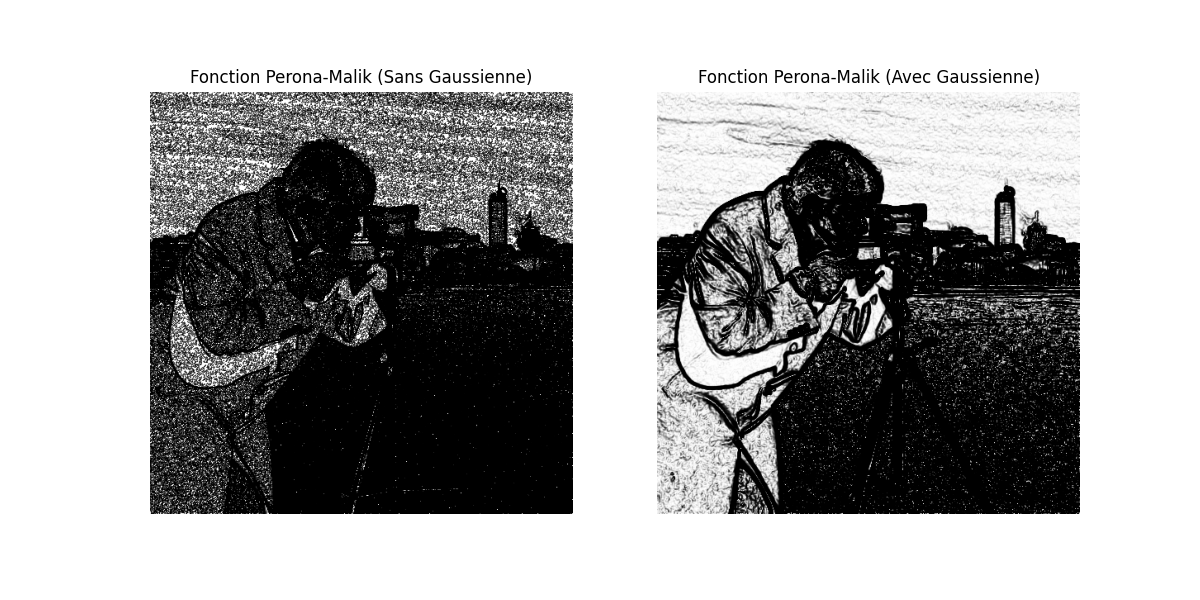
\includegraphics[trim=100 70 100 50, clip, width=\textwidth]{img/perona_malik_function_comparison.png}
      \caption{Fonction de Perona-Malik en fonction de la norme du gradient de l'image initiale avec et sans gaussienne.}
      \label{fig:perona_malik_function}
    \end{figure}
  \end{minipage}
\end{figure}
Nous observons que la fonction de Perona-Malik sans gaussienne est plus sensible aux variations du gradient, ce qui peut entraîner un lissage excessif des zones homogènes. En revanche, la fonction avec gaussienne est plus douce et préserve mieux les détails de l'image tout en réduisant le bruit.

\section{Conclusion et perspectives}
Ce projet a permis d'explorer la résolution d'équations différentielles ordinaires et ses applications. Un solveur Cauchy a été implémenté en utilisant diverses méthodes d'intégration numérique pour résoudre des équations différentielles. Cet algorithme a été appliqué à la modélisation de l'évolution de la population d'un ensemble d'individus ainsi qu'au filtrage d'images via l'équation de la chaleur et le filtre de Perona et Malik.\\
Des résultats intéressants ont été obtenus, bien que des problèmes de convergence et de stabilité aient émergé avec certaines méthodes d'intégration numérique. Ces difficultés ont été surmontées en ajustant les paramètres d'entrée et en optimisant la gestion de la mémoire dans le code.\\
Les solutions des équations différentielles ont montré des comportements variés selon les paramètres et les conditions initiales, mettant en évidence l'importance du choix des méthodes d'intégration numérique et de la compréhension des propriétés des équations pour garantir des résultats fiables.\\ \\
Pour approfondir cette étude, il serait pertinent d'explorer d'autres méthodes d'intégration numérique, comme Crank-Nicolson, et d'appliquer l'algorithme à des problèmes de modélisation différents. Une analyse plus poussée de l'impact des conditions initiales et des paramètres sur les solutions et leur dynamique pourrait également enrichir cette recherche.\\

%%%%%%%%%%%%%%%% Bibliography %%%%%%%%%%%%%%%%

\printbibliography
\end{document}